\documentclass[a4paper,11pt]{article}

\usepackage{mlsubmit}
\usepackage{assign-style}
\usepackage{scrextend}

\begin{document}
\setlength\parindent{0pt}

\initmlsubmision{2}{Gurpreet Singh}{150259}

\begin{mlsolution}

    \subsection*{Part 1}
    \begin{addmargin}{1.5em}
        No, name is not a useful attribute in learning a decision tree as splitting on this attribute will have no gain. Non-statistically speaking, there is a lot of variance in the attribute itself, and it will be very inefficient to decide on the basis of name as it can often be a newly observed value.
    \end{addmargin}

    \subsection*{Part 2}
    \begin{addmargin}{1.5em}
        It is not possible to classify the data given perfectly. Looking at data \#4 and \#6, they have the same values for all fields except for `name', however have different target values. Since we shall not use `name' as a decision classifier (as discussed in Part A), therefore we can say that is is not possible to classify the data perfectly.
    \end{addmargin}

    \subsection*{Part 3}
    \begin{addmargin}{1.5em}

        \begin{figure}[h!]\label{tree:q1}
            \center%
            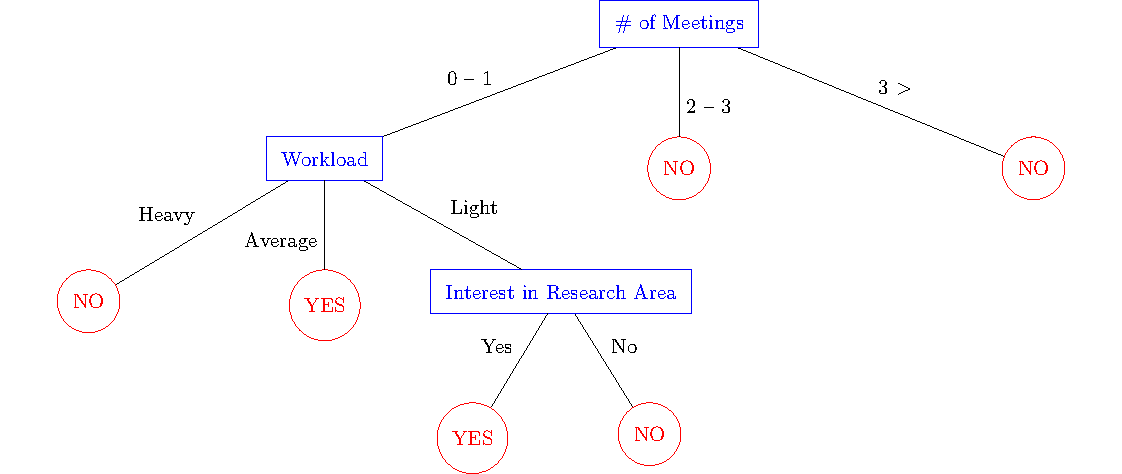
\includegraphics{q1-tree.pdf}
            \caption{ID3 Tree for the given data}
        \end{figure}

        ID3 is a greedy strategy to generate decision trees using Information Gain. The information gain at each level/depth is mentioned below

        \subsubsection{Level 1}
        \begin{addmargin}{1.5em}

            \textbf{Entropy} $S = 0.9183$ \br%

            \textbf{IG:\ Size of Research Group} $ = S - 0.2600 - 0.2667 - 0.3237 = 0.0679$

            \textbf{IG:\ Interest in Research Area} $ = S - 0.2667 - 0.6199 = 0.0317$

            \textbf{IG:\ Workload} $ = S - 0.4000 - 0.2163 - 0.2406 = 0.0614$

            \textbf{IG:\ Number of Meetings} $ = S - 0.6667 = 0.2516$ \br%

            Clearly the attribute \textit{Number of Meetings} provides the most IG, and hence we use this attribute to split at the first level.

        \end{addmargin}

        \subsubsection{Level 2 --- Number of Meetings}
        \begin{addmargin}{1.5em}

            Possible distictions --- `$0 - 1$', `$2 - 3$', `$> 3$' \br%

            Since for `$2 - 3$' and `$> 3$', all labels are `No' (\textbf{i.e.} entropy is $0$), hence we do need to split here, and we add leaf nodes. \br%

            For the samples remaining with value `$0 - 1$' of the attribute \textit{Number of Meetings}, we will further extend the decision tree. \br%

            \textbf{Extropy} $S = 1$ \br%

            \textbf{IG:\ Size of Research Group} $ = S - 0.0000 - 0.4000 - 0.4855 = 0.1145$

            \textbf{IG:\ Interest in Research Area} $ = S - 0.2755 - 0.6897 = 0.0348$

            \textbf{IG:\ Workload} $ = S - 0.0000 - 0.0000 - 0.3610 = 0.6390$
            \br%

            Clearly the attribute \textit{Workload} gives the highest gain, and hence we use this attribute to further construct the decision tree.

        \end{addmargin}

        \subsubsection{Level 3 --- Workload}
        \begin{addmargin}{1.5em}

            Possible distinctions --- `Light', `Average', `Heavy' \br%

            Since there is purity in the samples with `Average' and `Heavy' value in the \textit{Workload} attribute (\textit{i.e.} entropy is 0), we do not split further in this case. Therefore we are only left with two samples, which have the value `Light'. \br%

            \textbf{Entropy} $S = 1$ \br%

            \textbf{IG:\ Size of Research Group} $ = S - 1.0000 = 0.0000$

            \textbf{IG:\ Interest in Research Area} $ = S - 0.0000 = 1.0000$ \br%

            Hence we further split using \textit{Interest in Research Area} attribute. Since there is only one sample per distinction, we cannot split further. Hence we have the decision tree showed in Figure~\ref{tree:q1}

        \end{addmargin}

    \end{addmargin}

\end{mlsolution}

\begin{mlsolution}

    \begin{qsection}{Notations}

        \textbf{L:} Represents total number of items \br%

        \textbf{N:} Represents total number of users \br%

        \textbf{D:} Represents length of feature vector for every user \textit{i.e.} length of $\vx^n$ \br%

        \textbf{K:} $2^L$

    \end{qsection}

    \begin{qpart}{1}

        Any user can select any number of items. The probability of selecting an item for a user is represented by a logistic expression.

        \begin{equation}
            P(\mu_l \pipe \vx^n, \vw_l) = \sigmoid{\dotp{\vw_l}{\vx^n}}^{\mu_l} \bpara{1 - \sigmoid{\dotp{\vw_l}{\vx^n}}}^{(1 - \mu_l)}
            \label{eq:pr_item}
        \end{equation} \br%

        \qnote{$\sigma \bpara{x}$ represents the sigmoid function} \br%

        The equation~\ref{eq:pr_item} represents the probability of user $n$ selecting item $l$ \textit{i.e.} $\mu_l = 1$ if item $l$ has been selected, $0$ otherwise. We assume that the probability is represented by the same expression for all users and is independent, since all users are independent and are represented by their feature vector $\vx^n$. \br%

        It is clear that there are $K$ possible subsets of the items. Hence the user can choose any one of the subsets. Let these subsets be denoted by $S_k$. Hence the powerset of the items set is $\bset{S_k}_{k = 1}^{K}$. Now, we can write the expression for a user selecting a subset of items.

        \begin{equation}
            P(S_k \pipe \vx^n, \bset{\vw_l}_{l = 1}^{L}) = \prod_{l \in S_k} P(\mu_l = 1 \pipe \vx^n) \prod_{l \notin S_k} P(\mu_l = 0 \pipe \vx^n)
            \label{eq:pr_subset}
        \end{equation} \br%

        Here, $\bset{\vw_l}_{l = 1}^{L}$ is a parameter for the model. \br%

    Now we define our latent variable $z^n \in \brac{K}$. This is the index of the subset of items, in the powerset, that the user $n$ has chosen \textit{i.e.} $z^n = k$ represents the subset $S_k$. Hence, we can define the conditional probability of $z^n$ as follows

        \begin{equation}
            P(z^n \pipe \vx^n, \bset{\vw_l}_{l = 1}^{L}) = \prod_{k = 1}^{K} P{(S_k \pipe \vx^n, \bset{\vw_l}_{l = 1}^{L})}^{\is{z^n = k}}
            \label{eq:pr_latent}
        \end{equation} \br%
        
        We also define a function $h:\brac{K} \rightarrow \R$ such that

        \begin{equation}
            h(z^n) = \sum_{l \in S_{z^n}} c_l
            \label{eq:fn_h}
        \end{equation} \br%

        We can now write the expression for the conditional probablity of our output variable $b^n$ as follows

        \begin{equation}
            b^n \pipe z^n, \sigma \sim \ND{b^n \pipe h(z^n), \sigma^2}
            \label{eq:pr_out}
        \end{equation} \br%

        \qnote{$b^n \pipe z^n, \sigma \quad \sim \quad b^n \pipe z^n, \vx^n, \sigma$}. This is because once we assume a value of $z^n$, $\vx^n$ no longer plays a role in the conditional probability \br%

        \qnote{We can collectively define $\sigma, \bset{\vw_l}_{l = 1}^{L}$ as $\vTheta$}

    \end{qpart}

    \begin{qpart}{2}

        We can represent the Complete Likelihood (CLE) as follows

        \begin{equation*}
            CLE \sim \vb, \vz \pipe \vX, \vTheta
        \end{equation*}

        Since all users are independent, we can write the above as follows

        \begin{equation}
            P(\vb, \vz \pipe \vX, \vTheta)  &=  \prod_{n = 1}^{N} P(b^n, z^n \pipe \vx^n, \vTheta)
            \label{eq:pr_cle}
        \end{equation}
        
        Using bayes rule, we can further expand this probability term

        \begin{align*}
            P(b^n, z^n \pipe \vx^n, \vTheta)        &=  P(b^n \pipe z^n, \vTheta) P(z^n \pipe \vx^n, \vTheta) \\
            \implies P(\vb, \vz \pipe \vX, \vTheta) &= \prod_{n = 1}^{N} P(b^n \pipe z^n, \vTheta) P(z^n \pipe \vx^n, \vTheta)
        \end{align*}

        We can also write the Complete Log Likelihood (CLL) from the above exporession

        \begin{equation}
            CLL = \sum_{n = 1}^{N} \log\bpara{P(b^n \pipe z^n, \sigma)} + \sum_{n = 1}^{N} \log\bpara{P(z^n \pipe \vx^n, \bset{\vw_l}_{l = 1}^{L})}
            \label{eq:pr_cll}
        \end{equation}
        
    \end{qpart}

    \begin{qpart}{3}
        
        Since directly finding $\vTheta_{MLE}$ is a NP hard problem, therefore, we use alternating optimization to find out an approximate MLE estimate of $\vTheta$. The algorithm for alternating optimization is as follows

        \begin{qalgorithm}[0.9\textwidth]{h!}{\textit{Alternating Optimization --- Hard Assignment}}
            
            Initialize $\vTheta_{MLE}$ to $\vTheta_{MLE}^0$
            
            while \textbf{no convergence}:
            \begin{addmargin}{1.5em}
                
                \begin{align*}
                    \shortintertext{\textbf{Update} $\vz$}
                    \forall \quad n \in \brac{N}: \quad &z^n    &=  \quad&  \argmax_{k} P(z^n = k \pipe b^n, \vx^n, \vTheta) \\
                                                                &&= \quad&  \argmax_{k} \log\bpara{P(b^n, z^n = k \pipe \vx^n, \vTheta)} \\
                                                                &&= \quad&  \argmin_{k} \bpara{b^n - h(k)}^2 - \sum_{l \in S_k} \log\bpara{\sigmoid{\dotp{\vw_l}{\vx^n}}} - \sum_{l \notin S_k} \log\bpara{1 - \sigmoid{\dotp{\vw_l}{\vx^n}}}
                    \\
                    \shortintertext{\textbf{Update MLE of} $\vTheta$}
                    &\sigma_{MLE}                               &=  \quad&  \argmax_{\sigma} CLL \\
                                                                &&= \quad&  \argmax_{\sigma} \log\bpara{P(\vb \pipe \vz, \sigma)} \\
                                                                &&= \quad&  \sqrt{\frac{1}{N} \sum_{n = 1}^{N} {(b^n - h(z^n))}^2} \\
                    \\
                    \forall \quad l \in \brac{L}: \quad &\vw_l_{MLE}    &=  \quad&  \argmax_{\vw_l} CLL \\
                                                                        &&= \quad&  \argmax_{\vw_l} \log\bpara{P(\vz \pipe \vX, \bset{\vw_l}_{l = 1}^{L})} \\
                                                                        &&= \quad&  \argmax_{\vw_l} \sum_{n = 1}^{N} \bbpara{\is{l \in S_{z^n}} \log\bpara{\sigmoid{\dotp{\vw_l}{\vx^n}}} + \is{l \notin S_{z^n}} \log\bpara{1 - \sigmoid{\dotp{\vw_l}{\vx^n}}}}
                \end{align*}

            \end{addmargin}

        \end{qalgorithm}

        \begin{qsubsection}{Time Complexity Analysis}

            We need to compute $\dotp{\vw_l}{\vx^n}$ for all items and users. It is optimal to save this and store it before starting the updation steps. This can be done in $\bigO(NLD)$ steps. We can also compute the values of the isomorphism $h$ for all subsets \textit{i.e.} compute $h(k)$ for all k. This needs to be done only once, and can be done in the preprocessing part. Hence we need not add the time for this in the iteration time. \br%

            Therefore, for all $z^n$ updations, we need to check for all subsets, and we need to compute probability of the user choosing that subset. Since we have already computed some of the terms, we will only require $\bigO(NKL)$ time for this updation. \br%

            The MLE update of $\sigma$ requires only $\bigO(N)$. \br%

            For the MLE estimate of $\vw_l$, we need to find the MLE estimate of a logistic expression, using function approximation. As mentioned, we can assume that each FA takes $\bigO(ND)$ time, therefore, we can do this step in $\bigO(NLD)$.

            Hence the total time for each updation is $\bigO(NLD + N + NKL)$. Since $L \le D$, we can clearly say that this is bounded by $\bigO(NKD)$ or $\bigO(2^L ND)$.
            
        \end{qsubsection}

    \end{qpart}

    \begin{qpart}{4}

        In case of soft assignment, we cannot directly use the mode of the posterior (point estimate) as an estimate of $\vz$. Therefore, we take the expected value of $\vz$ and use EM algorithm to compute the MLE estimate of $\vTheta$. \br%

        It will be easier to use the one-hot representation of the $z^n$, as we will simply assign the expected probability in the $k^{th}$ index of the user buying the $k^{th}$ subset of items. This is similar to the soft k-means algorithm. \br%
        
        \qnote{$\vz^n$ represents the one-hot representation, whereas $z^n$ represents the numerical value}

        \begin{qalgorithm}[0.9\textwidth]{h!}{\textit{Alternating Optimization --- Soft Assignment}}

            
            Initialize $\vTheta_{MLE}$ to $\vTheta_{MLE}^0$
            
            while \textbf{no convergence}:
            \begin{addmargin}{1.5em}
                
                \begin{align*}
                    \shortintertext{\textbf{Update} $\vz$}
                    &\forall \quad n \in \brac{N}: &&&\\
                    &\forall \quad k \in \brac{K}: & \E{\vz^n_k}    \quad   &=   \quad  \frac{P(S^k | \vx^n, \bset{\vw_l}_{l = 1}^{L}) \ND{b^n | h(k), \sigma^2}}{\sum_{\pr{k} = 1}^{K} P(S^\pr{k} | \vx^n, \bset{\vw_l}_{l = 1}^{L}) \ND{b^n | h(\pr{k}), \sigma^2}} \\
                    \\
                    \shortintertext{\textbf{Update MLE of} $\vTheta$}
                    &&\sigma_{MLE}                                  \quad   &=   \quad  \argmax_{\sigma} \E{CLL} \\
                                                                            &&&= \quad  \argmax_{\sigma} \E{\log\bpara{P(\vb \pipe \vZ, \sigma)}} \\
                                                                            &&&= \quad  \sqrt{\frac{1}{N} \sum_{n = 1}^{N} \E{\bpara{b^n - h(z^n)}^2}} \\
                                                                        &&&= \quad  \sqrt{\frac{1}{N} \sum_{n = 1}^{N} \bbpara{\para{b^n}^2 - 2 \sum_{k = 1}^{K} \vz_k^n \, h(k) + \sum_{k = 1}^{K} \vz_k^n \, {h(k)}^2}}\\
                    \\
                    &\forall \quad l \in \brac{L}: & \vw_l_{MLE}    \quad   &=   \quad  \argmax_{\vw_l} \E{CLL} \\
                                                                            &&&= \quad  \argmax_{\vw_l} \E{\log\bpara{P(\vZ \pipe \vX, \bset{\vw_l}_{l = 1}^{L})}} \\
                                                                            &&&= \quad  \argmax_{\vw_l} \E{\log\bbpara{\prod_{n = 1}^{N} \prod_{k = 1}^{K} \bbbrac{\prod_{\pr{l} \in S_k} \sigmoid{\dotp{\vw_{\pr{l}}}{\vx^n}} \prod_{\pr{l} \notin S_k} \bpara{1 - \sigmoid{\dotp{\vw_{\pr{l}}}{\vx^n}}}}^{\vz_k^n}}} \\
                                                                            &&&= \quad  \argmax_{\vw_l} \sum_{k: l \in S_k} \sum_{n = 1}^{N} \vz_k^n \sigmoid{\dotp{\vw_{\pr{l}}}{\vx^n}} + \sum_{k: l \notin S_k} \sum_{n = 1}^{N} \vz_k^n \bpara{1 - \sigmoid{\dotp{\vw_{\pr{l}}}{\vx^n}}}
                \end{align*}

            \end{addmargin}
            
        \end{qalgorithm}

    \end{qpart}

\end{mlsolution}

\begin{mlsolution}

    \begin{qpart}{1}

        We have the optimization problem $(P1)$ as follows

        \begin{align*}
            \label{eq:P1}
            \min_{\vw, \bset{\xi_i}}    &   \norm{\vw}_2^2 + \sum_{i = 1}^{n} \xi_i^2 \tag*{(P1)} \\
            &   s.t. \forall i \in \brac{n} \quad 1 - y^i \dotp{\vw}{\vx^i} \le \xi_i \\
            &   \xi_i \ge 0
        \end{align*} \br%

        Now consider an optimization problem $(P2)$, which is similar to the optimization problem given in equation~\ref{eq:P1}, except that we do not have the condition $\xi_i \ge 0$ for any $i \in \brac{n}$. Clearly, the convexity still holds, and hence we will have a solution for $(P2)$. \br%

        Consider this solution to be $\vw_0, \bset{\xi_i^0}$. If we do not have any $k \in \brac{n}$ such that $\xi_k^0 < 0$. Then we can safely claim that the solution for both the optimization problems $(P1)$ and $(P2)$ is the same. Otherwise, we will have at least one $k \in \brac{n}$ such that the condition holds, \textit{i.e.} $\xi_k^0 < 0$. Since this is a solution of the $(P2)$, we can say that this satisfies the condition $1 - y^k \dotp{\vw}{\vx^k} \le \xi_k^0$.

        Now consider the pair $\vw, \bset{\xi_i^1}$ where 

        \begin{align*}
            \xi_i^1 = \begin{cases}
                \xi_i^0     &   if i \ne k \\
                0           &   if i = k
            \end{cases}
        \end{align*} \br%

        Since $0 > \xi_k^0$, we can say that it follows all constraints of $(P2)$ and $0 < \para{\xi_k^0}^2$. For all other $\xi_i^1$, they are the same and hence do not change anything (since all $\xi_i$ are independent). Hence, we can say that $w, \bset{\xi_i^1}$ is a solution of $(P2)$, and $val(P2, \bpara{w, \bset{\xi_i^1}}) < val(P2, \bpara{w, \bset{\xi_i^1}})$. \br%

        However, since $w, \bset{\xi_i^0}$ was claimed to be a valid solution, this is not possible. Hence the claim that can exist a $k \in \brac{n}$ such that $\xi_k^0 < 0$ is false. Hence, the solution of $(P2)$ is always the same as that of $(P1)$, which suggests that the second constraint is vacuous.

    \end{qpart}

    \begin{qpart}{2}

        \begin{align*}
            \min_{\vw, \bset{\xi_i}}    &   \norm{\vw}_2^2 + \sum_{i = 1}^{n} \xi_i^2 \tag*{(P1)} \\
            &   s.t. \forall i \in \brac{n} \quad 1 - y^i \dotp{\vw}{\vx^i} \le \xi_i \quad \text{and} \quad - \xi_i \le 0
        \end{align*} \br%

        We can convert this problem to an unconstrained optimization problem using Langrange Multipliers.

        \begin{align*}
            & \min_{\vw, \bset{\xi_i}} \max_{\vlambda, \vgamma \ge \vzero} \norm{\vw}_2^2 + \sum_{i = 1}^{n} \xi_i^2 + \sum_{i = 1}^{n} \lambda_i \bpara{1 - y^i \dotp{\vw}{\vx^i} - \xi_i} - \sum_{i = 1}^{n} \gamma_i \xi_i \tag*{(P1)}\\
            \label{eq:P1l}
        \end{align*} \br%

    \end{qpart}

    \begin{qpart}{3}

        We can convert the optimization problem $(P1)$ given in equation~\ref{eq:P1l} to a dual problem. Assuming strong duality, we can switch the optimization variables.

        \begin{align*}
            & \max_{\vlambda, \vgamma \ge \vzero} \min_{\vw, \bset{\xi_i}} \norm{\vw}_2^2 + \sum_{i = 1}^{n} \xi_i^2 + \sum_{i = 1}^{n} \lambda_i \bpara{1 - y^i \dotp{\vw}{\vx^i} - \xi_i} - \sum_{i = 1}^{n} \gamma_i \xi_i \tag*{(P1)}\\
        \end{align*} \br%

        Now using this, we can first optimize based on the inner optimization (using differentiation). That is, we can partially differentiate w.r.t.\ to $\vw$ and $\bset{\xi_i}$ separately, in order to obtain a dual problem.

        \begin{align*}
            \frac{\partial P1}{\partial \vw}    =& \quad 2\vw - \sum_{i = 1}^{n} \lambda_i y^i \vx^i = 0 \\
            \implies& \quad \pr{\vw} = \frac{1}{2} \sum_{i = 1}^{n} \lambda_i y^i \vx^i \\
            \\
            \frac{\partial P1}{\partial \xi_k}  =& \quad 2\xi_k - \lambda_k - \gamma_i = 0 \\
            \implies& \quad \pr{\xi_k} = \frac{\lambda_k + \gamma_i}{2}
        \end{align*} \br%

        Hence, we can replace these values in the optimization problem, while solving the inner optimization problem.

        \begin{align*}
            & \max_{\vlambda, \vgamma \ge 0} \quad  \norm{\pr{\vw}}_2^2 + \sum_{i = 1}^{n} \pr{\xi_i}^2 + \sum_{i = 1}^{n} \lambda_i \bpara{1 - y^i \dotp{\pr{\vw}}{\vx^i} - \pr{\xi_i}} - \sum_{i = 1}^{n} \gamma_i \pr{\xi_i} \\
            =& \max_{\vlambda, \vgamma \ge 0} \quad  \norm{\frac{1}{2} \sum_{i = 1}^{n} \lambda_i y^i \vx^i}_2^2 + \frac{1}{4} \sum_{i = 1}^{n} \bpara{\lambda_i + \gamma_i}^2 - \sum_{i = 1}^{n} \lambda_i - \sum_{i = 1}^{n} \lambda_i y^i \dotp{\frac{1}{2} \sum_{j = 1}^{n} \lambda_j y^j \vx^j}{\vx^i} - \frac{1}{2} \sum_{i = 1}^{n} \bpara{\lambda_i + \gamma_i}^2 \\
            =& \max_{\vlambda, \vgamma \ge 0} \quad  \norm{\frac{1}{2} \sum_{i = 1}^{n} \lambda_i y^i \vx^i}_2^2 - \frac{1}{2} \sum_{i = 1}^{n} \sum_{j = 1}^{n} \lambda_i \lambda_j y^i y^j \dotp{\vx^j}{\vx^i} - \frac{1}{4} \sum_{i = 1}^{n} \bpara{\lambda_i + \gamma_i}^2 - \sum_{i = 1}^{n} \lambda_i
        \end{align*}

        We can expand the first term as

        \begin{align*}
            & \norm{\frac{1}{2} \sum_{i = 1}^{n} \lambda_i y^i \vx^i}_2^2 = \frac{1}{4} \norm{\sum_{i = 1}^{n} \lambda_i y^i \vx^i}_2^2 \\
            \implies & \norm{\frac{1}{2} \sum_{i = 1}^{n} \lambda_i y^i \vx^i}_2^2 = \frac{1}{4} \sum_{i = 1}^{n} \sum_{j = 1}^{n} \lambda_i \vlambda_j y^i y^j \dotp{\vx^i}{\vx^j}
        \end{align*}

        Replacing back in the original equation

        \begin{align*}
            =& \max_{\vlambda, \vgamma \ge \vzero} \quad  - \frac{1}{4} \sum_{i = 1}^{n} \sum_{j = 1}^{n} \lambda_i \lambda_j y^i y^j \dotp{\vx^j}{\vx^i} - \frac{1}{4} \sum_{i = 1}^{n} \bpara{\lambda_i + \gamma_i}^2 - \sum_{i = 1}^{n} \lambda_i \\
        \end{align*}

        We can alter this optimization problem by multiplying with $-4$ and inverting the optimizing condition. Hence the dual can be given as follows

        \begin{align*}
            & \min_{\vlambda, \vgamma \ge \vzero} \vlambda^T Q \vlambda + \sum_{i = 1}^{n} \bpara{\lambda_i + \gamma_i}^2 - 4 \lambda_i \tag*{(D1)} \\
            \shortintertext{where}
            & Q_{ij} = y^i y^j \dotp{\vx^i}{\vx^j}
        \end{align*}

        Note that $\lambda_i, \gamma_i \ge 0$ for all $i \in \brac{n}$. Hence, $\bpara{\lambda_i + \gamma_i}^2 \ge \bpara{\lambda_i}^2$, hence it is very trivial to see that $\gamma_i = 0$ for all $i \in \brac{n}$. Therefore, we can further simplify the dual as follows

        \begin{align*}
            \min_{\vlambda \ge \vzero} \vlambda^T Q \vlambda + \sum_{i = 1}^{n} \bpara{\lambda_i^2 - 4 \lambda_i} \tag*{(D1)} \\
            \shortintertext{where}
            Q_{ij} = y^i y^j \dotp{\vx^i}{\vx^j}
        \end{align*}
        

    \end{qpart}

    \begin{qpart}{4}

        Let us state the original dual problem.

        \begin{align*}
            \min_{\valpha \in \brac{0, C}^n} \valpha^T Q \valpha - \sum_{i = 1}^{n} \valpha_i
        \end{align*}

        The main difference that seems to be there between the two objectives is that the dual variable (each value) in the original problem is upper bounded by a constant $C$. \br%

        It seems that the dual variable in $(D1)$ has no upper bound, however there is still a tradeoff between the high and low values of our dual variable. Consider $\vlambda > 2$. In this case, the second term will become positive. Hence, we do not want very hight values of $\vlambda$. Looking at the primal problem of the original SVM, we can say that in our case (by similarity of terms), C = 2. Hence we are trying to keep the value of $\lambda$ within the range $\brac{0, C}^n$, however it is a loose bound. \br%

        Therefore, the only difference is that in the original SVM problem, we have a strict upper bound on the value of the dual variable, whereas in our case, the upper bound is loose, but still existant.

    \end{qpart}

    \begin{qpart}{5}

        \textbf{No}. From our approach, we have proved that $\xi_i < 0$ only increases the value of the objective function while $\xi_i = 0$ is a solution, and hence the lower bound is vacuous, however, this is not the case with the original SVM.\ In the original problem, we are hoping to get negative values of $\xi_i$ which would mean that we are giving weightage to the points which are far from the margin, which is not a correct optimization problem, as it essentials ignores the large margin problem. Hence, in that case, we need to explicitly add the lower bound.

    \end{qpart}

\end{mlsolution}

\begin{mlsolution}

    \begin{qpart}{3}

        The averaging trick did not give better results in the case of Vanilla Gradient Descent. Determined on the basis of held-out validation, the model with w\_bar gave slightly lesser accuracy as well as higher value of the objective function for all iterations. This is evident in the validation data provided in figure~\ref{fig:val}
        
    \end{qpart}

    \begin{qpart}{4}

        I took $h(n)$ as $\frac{1}{n}$, as it allows for averaging the sum of the support vectors. As for the constant multiplied to $\frac{h(n)}{\sqrt{t + 1}}$, I used held-out validation to find the fastest converging as well as the one with the best accuracy. Amongst the set of values $\bset{1, 8, 16, 32, 64, 100}$, the best value came out to be 32. \br%

        Hence, the best value of $\eta$ for me was $\frac{32}{n \sqrt{t + 1}}$. This is inspite of the fact that initially the value of the objective function increases \textit{i.e.} the objective function first diverges, then converges. Using a smaller value of the constant (5) avoids this problem, however gives lower final accuracy and slower convergence.

        \clearpage

        \begin{figure}[h!]
            \centering
            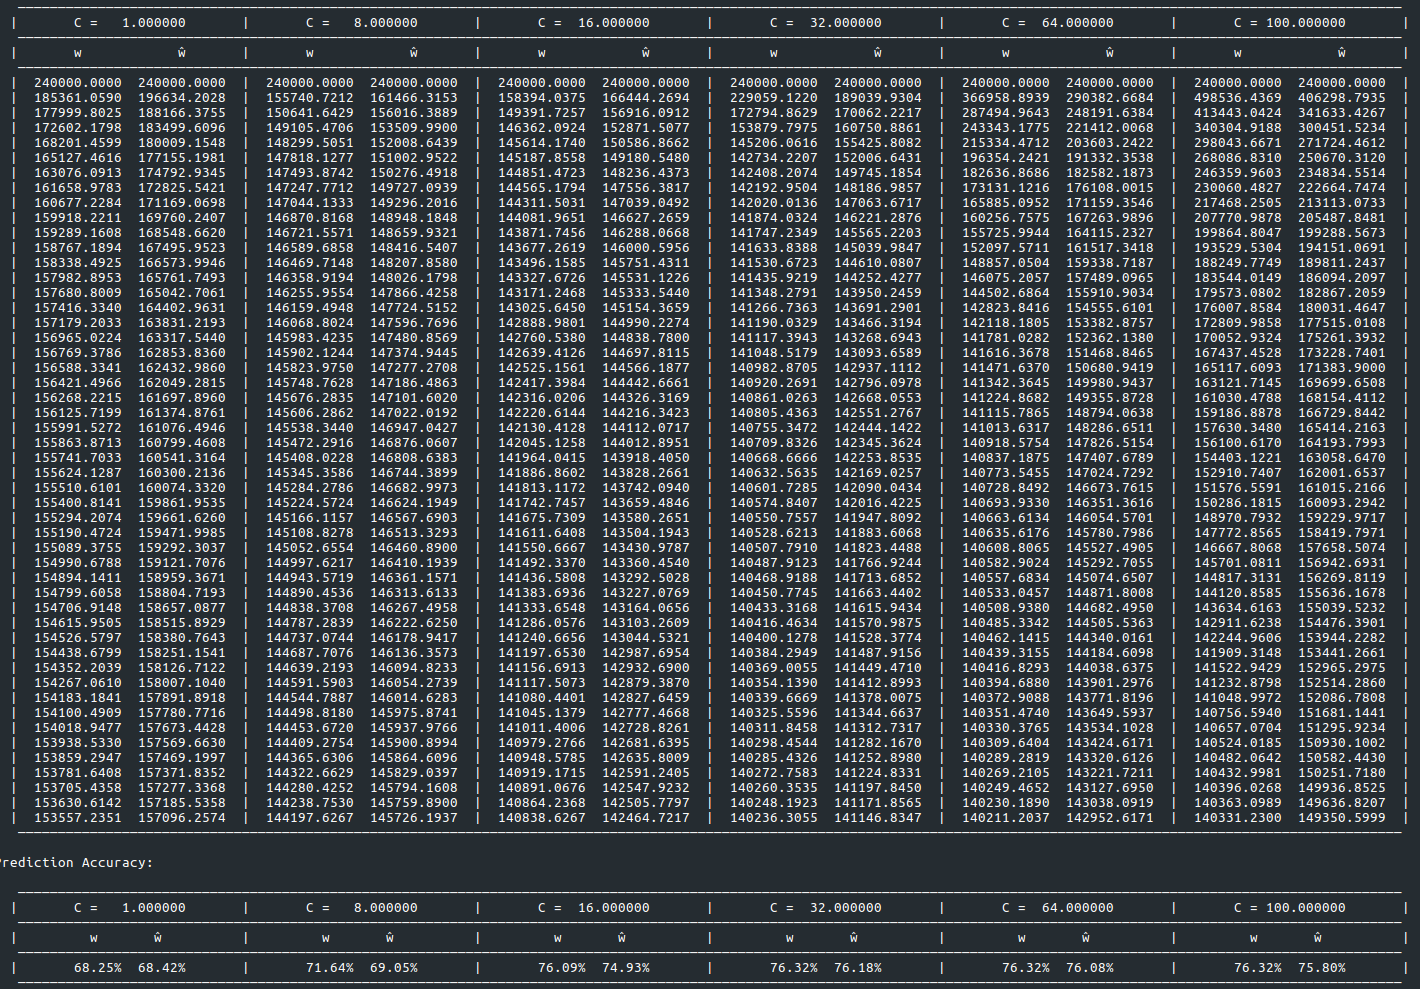
\includegraphics[width=\textwidth]{validation_data.png}
            \caption{Cross validation data for some values of $\eta$}
            \label{fig:val}
        \end{figure}

    \end{qpart}

    \begin{qsection}{Part 5 and Part 6}

        The plots have been generated after running GD and SCD on the complete training dataset \textit{i.e.} 300K examples. \br%

        For GD, I have taken $n\_iter = 2000$ and $spacing = 10$, whereas for SCD, $n\_iter = 100000$ and $spacing = 5000$. \br%

        \begin{figure}[h!]\label{fig:q4-clock}
            \centering
            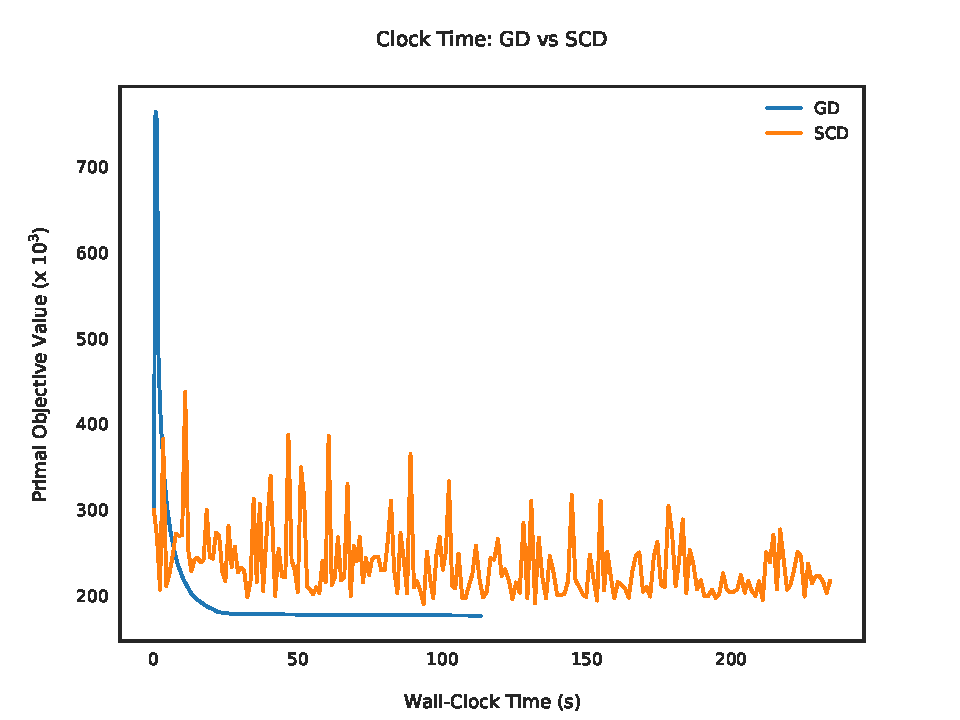
\includegraphics{q4-plot-clocktime.pdf}
            \caption{Clock Time Analysis of Gradient Descent vs Stochastic Coordinate Descent}
        \end{figure}
        
        \begin{figure}[h!]
            \centering
            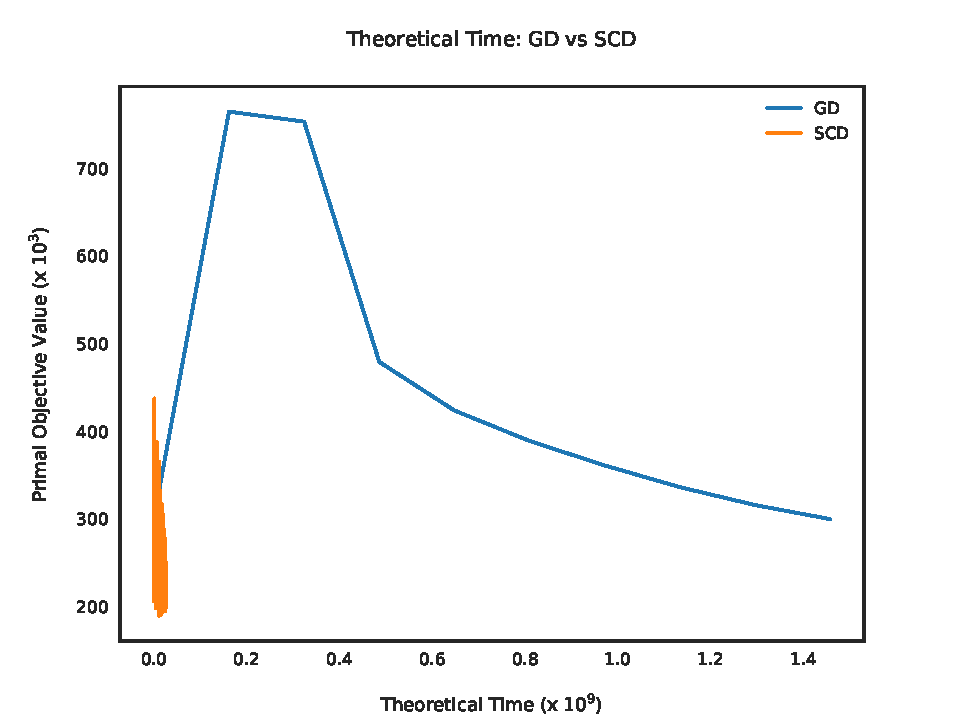
\includegraphics{q4-plot-theoreticaltime.pdf}
            \caption{Theoretical Time Analysis of Gradient Descent vs Stochastic Coordinate Descent}
        \end{figure}
 
        \begin{figure}[h!]
            \centering
            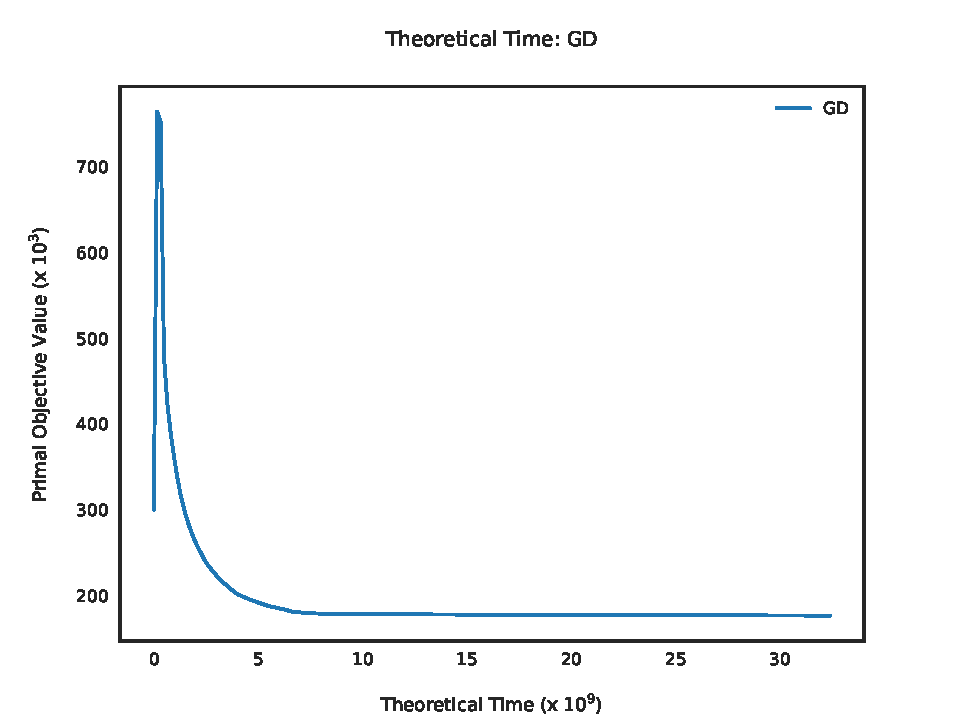
\includegraphics[width=0.48\textwidth]{q4-plot-theoreticaltime-GD.pdf}
            \hfill%
            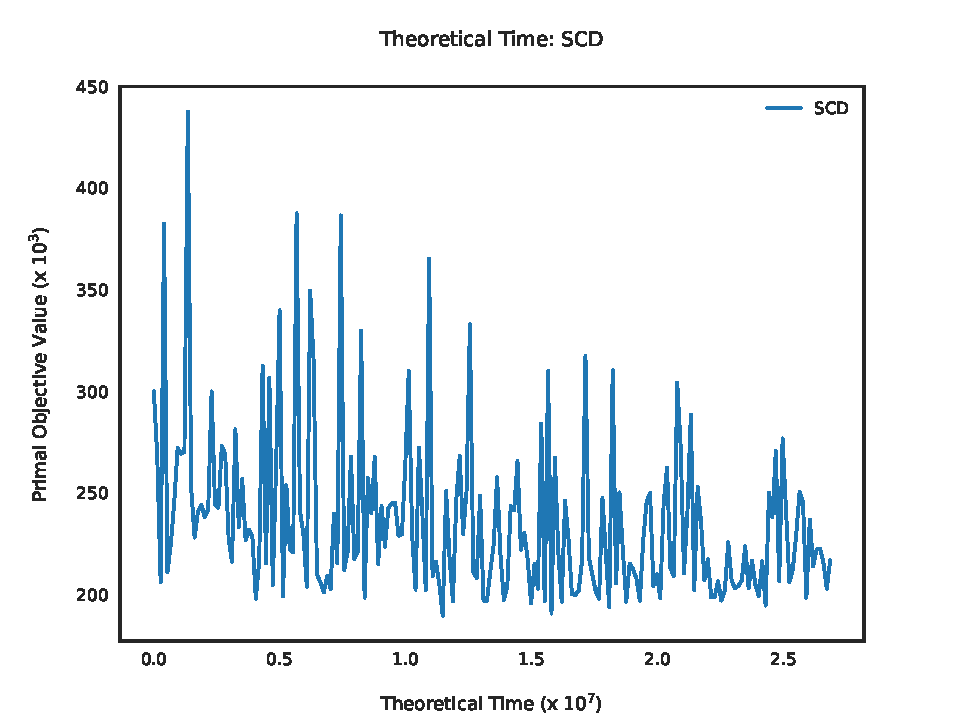
\includegraphics[width=0.48\textwidth]{q4-plot-theoreticaltime-SCD.pdf}
            \caption{Theoretical Time Analysis of (a) Gradient Descent and (b) Stochastic Coordinate Descent}
        \end{figure}

        From the figures, it is evident that Gradient Descent gives lower objective function value, and thus a better solution, wheras SCD gives a lot of fluctuations. However, this is not actually the case. In the case of SCD, there is obviously a tradeoff between the objective value and margin, and the speed. The SCD method very quickly gives good accuracy, wheras the GD takes much more time to give the same accuracy.

        Also, looking at the theoretical plots, it seems that the work done by SCD is much smaller than that of GD\. However, this is not in relevance to the observed time for the same set of training data. The theoretical time and wall-clock time are definitely correlated, however, it seems that there is a lot more overhead on $\bigO(1)$ operations than expected by the work done per iteration in the SCD method. The difference in the methods might become more relevant in case of much larger values of the size of the dataset used.

    \end{qsection}

\end{mlsolution}

\end{document}
